\documentclass[10pt,a4paper]{report}
\usepackage[left=3.00cm, right=1.00cm, top=2.00cm, bottom=2.00cm, nohead, footskip=7mm]{geometry}
\usepackage[14pt]{extsizes}

\usepackage[utf8]{inputenc}
\usepackage[T1]{fontenc}
\usepackage{amsmath}
\usepackage{amsfonts}
\usepackage{amssymb}
\usepackage{pdfpages}

\usepackage[russian]{babel}

% Отступ абзаца
\usepackage{indentfirst}
\setlength{\parindent}{1.5cm} 

% Межстрочный интервал
\usepackage{setspace}
\onehalfspacing % интервал 1.5

% Вставка изображений
\usepackage{graphicx}
\graphicspath{{schemes/}}

% Настройка оглавлений
\usepackage{titlesec}
\newcommand{\hsp}{\hspace{20pt}}
\titleformat{\chapter}[hang]{\large\bfseries}{\thechapter{. }}{0pt}{\large\bfseries}
\titlelabel{hlabel-formati}
\titlespacing{\chapter}{42pt}{-80pt}{12pt}
\titleformat{\section}[hang]{\large\bfseries}{\thesection{. }}{0pt}{\large\bfseries}
\titlespacing{\section}{42pt}{12pt}{5pt plus 5pt}

% Настройка списков
\usepackage{enumitem}
\setlist{nolistsep, itemsep=0.3cm,parsep=0pt,leftmargin=1.9cm}

% Настройка листингов
\usepackage{listings}
\lstset{
	language = python,
	extendedchars=\true,
	keepspaces=true,
	basicstyle=\small\sffamily,
	showstringspaces=\false,
	numbers=left,
	stepnumber=1,
	numbersep=5pt,
	frame=single,
	tabsize=2,
	captionpos=t,
	breaklines=true,
	breakatwhitespace=false,
	escapeinside={\#*}{*)}
}





\begin{document}
	
	\includepdf[pages=1]{report_word.pdf}
	%%%%%%%%%%%%%%%%%%%%%%%%%%%%%%%%%%%%%%%%%%%%%%%%%%%%%%%%%%	
	
	\tableofcontents
	\newpage

	%%%%%%%%%%%%%%%%%%%%%%%%%%%%%%%%%%%%%%%%%%%%%%%%%%%%%%%%%%	
	\chapter*{Введение}
	\addcontentsline{toc}{chapter}{Введение}
	Расстояние Левенштейна – минимальное количество редакционных операций, которые необходимы для превращения одной строки в другую. Существуют следующие редакционные операции:
	\begin{itemize}
	\item вставка символа;
	\item удаление символа;
	\item замена символа;
	\end{itemize}

	\parРасстояние Дамерау-Левенштейна также учитывает и операцию транспозиции – перестановки двух соседних символов местами.\\
	\parДанные расстояния имеют большое количество применений. Они используются для автокоррекции при выполнении поисковых запросов и печати на клавиатуре, а также в биоинформатике для сравнения генов, представленных в строковом формате.
	
	\newpage
	%%%%%%%%%%%%%%%%%%%%%%%%%%%%%%%%%%%%%%%%%%%%%%%%%%%%%%%%%%
	\chapter{Аналитическая часть}
	Целью лабораторной работы является реализация и сравнение алгоритмов поиска расстояний Левенштейна и Дамерау-Левенштейна.
	
	Выделены следующие задачи лабораторной работы:
	
	\begin{itemize}
	\item математическое описание расстояний Левенштейна 
	и Дамерау-Левенштейна;
	\item описание и реализация алгоритмов поиска расстояний;
	\item проведение замеров процессорного времени работы алгоритмов при различных размерах строк;
	\item оценка наибольшей используемой каждым алгоритмом памяти;
	\item проведение сравнительного анализа алгоритмов на основании экспериментов;
	\end{itemize}

	Задача по поиску расстояний заключается в нахождении такой последовательности операций, применение которых даст минимальный суммарный штраф. Штрафы операций:
	\begin{itemize}
	\item вставка (I) – 1;
	\item замена (R) – 1;
	\item удаление (D) – 1;
	\item совпадение (М) – 0;
	\item транспозиция (T) – 1;
	\end{itemize}
	
	Для решения данной проблемы используется рекуррентная формула вычисления расстояний. Пусть D(s1[1..i], s2[1..j]) – расстояние Левенштейна для подстроки s1 длиной i и s2 длиной j. Формула вычисления D:
	\begin{equation}
		\left\{ 
		\begin{array}{ll}
				j, & $если $ i = 0\\
				i, & $если $ j = 0\\
				
				min(D(s1[1..i],s2[1..j-1]) + 1, \\
				\qquad D(s1[1..i-1],s2[1..j]) + 1,\\
				\qquad D(s1[1..i-1],s2[1..j-1]) +
					\left\{\begin{array}{ll}
						0, & $если $ s1[i] = s2[j]\\
						0, & $иначе$
					\end{array} \right.
					
					)
		\end{array}
		\right.
	\end{equation}

	Аналогично рекуррентно представляется формула расстояния Дамерау-Левенштейна:
		\begin{equation}
		\left\{ 
		\begin{array}{ll}
			j, & $если $ i = 0\\
			i, & $если $ j = 0\\
			
			min(
			D(s1[1..i],s2[1..j-1]) + 1, \\
			\qquad D(s1[1..i-1],s2[1..j]) + 1,\\
			\qquad D(s1[1..i-1],s2[1..j-1]) + \left\{\begin{array}{ll}
											0, & $если $ s1[i] = s2[j]\\
											0, & $иначе$
											\end{array}\right. ,\\
			\qquad \left\{\begin{array}{ll}
			D(s1[1..i-2],s2[1..j-2]) + 1, $ если $ \left\{\begin{array}{ll}
													i > 1, j > 1 \\
													s1[i] = s2[j-1] \\
													s1[i-1] = s2[j]
													\end{array}\right. \\
			+\infty, $ иначе $
									
			\end{array}\right.
			)
		\end{array}
		\right.
	\end{equation}
	
	
	\newpage
	%%%%%%%%%%%%%%%%%%%%%%%%%%%%%%%%%%%%%%%%%%%%%%%%%%%%%%%%%%
	\chapter{Конструкторская часть}
	Рассмотрим алгоритмы поиска расстояний Левенштейна и Дамерау-Левенштейна для строк s1 и s2 с длинами в n1 и n2 соответственно.
	
	\section{Расстояние Левенштейна, матричный метод}
	Алгоритм матричного поиска расстояния Левенштейна основывается на вышеописанной рекуррентной формуле. Создаётся целочисленная матрица размерами (n1+1)x(n2+1). В каждой клетке [i][j] этой матрицы будет записано значение D(s1[1..i-1], s2[1..j-1]). В случае, когда i=1 или j=1 вместо строк s1 и s2 соответственно будут выступать пустые строки. Искомым расстоянием Левенштейна будет значение ячейки [n1+1][n2+1].
	
	Нахождение расстояний алгоритм начинает с заполнения первого столбца и первой строки, так как они являются базой для рекуррентной формулы. После этого производится построчное заполнение остальной части матрицы.
	
	Схема алгоритма приведена на рисунке 2.1.
	\begin{figure}[h]
		\begin{center}
			{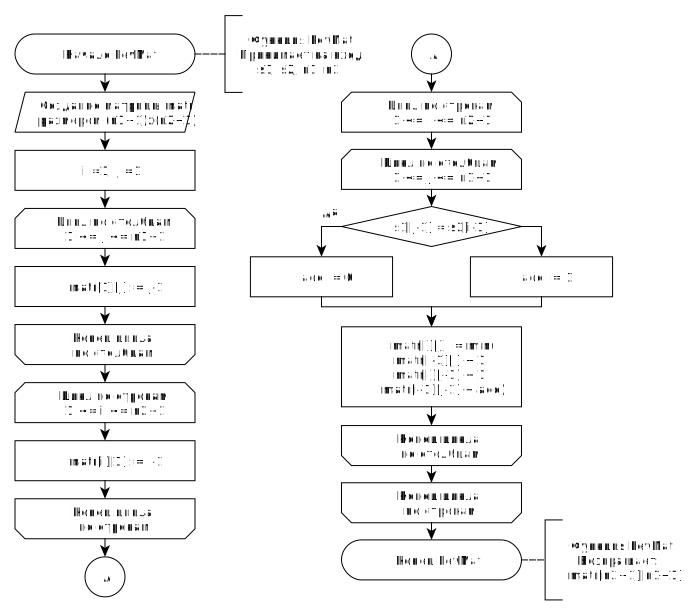
\includegraphics[scale = 0.7]{Lev_mat}}
			\caption{Алгоритм нахождения расстояния Левенштейна, матричный метод}
		\end{center}
	\end{figure}

	% //////////////
	\section{Расстояние Дамерау-Левенштейна, матричный метод}
	Алгоритм является модификацией вышеописанного способа нахождения расстояния Левенштейна. Дополнительно для ячейки [i][j] (i > 2, j > 2) рассматривается вариант перехода из клетки [i-2][j-2], при условии, что s1[i] = s2[j-1] и s1[i-1] = s2[j]. Искомым расстоянием Дамерау-Левенштейна также является значение ячейки [n1+1][n2+1].
	
	Схема алгоритма приведена на рисунке 2.2.
	\begin{figure}[h]
		\begin{center}
			{\includegraphics[scale = 0.55]{DamLev_mat}}
			\caption{Алгоритм нахождения расстояния Дамерау-Левенштейна, матричный метод}
		\end{center}
	\end{figure}


	% //////////////
	\section{Расстояние Левенштейна, рекурсивный метод}
	Данный алгоритм использует только рекурсивную формулу нахождения D(s1[1..i], s2[1..j]). Для этого используется рекурсивная функция, принимающая в себя строки s1, s2 и длины подстрок i, j. Функция вызывает функции для тех же строк, и длин: (i-1, j-1), (i-1, j) и (i, j-1), после чего возвращает минимальный из них.
	
	Схема алгоритма приведена на рисунке 2.3.
	\begin{figure}[h]
		\begin{center}
			{\includegraphics[scale = 0.7]{Lev_rec}}
			\caption{Алгоритм нахождения расстояния Левенштейна, рекурсивный метод}
		\end{center}
	\end{figure}

	% //////////////
	\section{Расстояние Левенштейна, рекурсивный метод с заполнением матрицы}
	В данном случае, в качестве основы используется алгоритм Дейкстры поиска расстояний до вершин в графе. Создаётся матрица размерами (n1+1)x(n2+1), все ячейки которой изначально заполнены значением +$\infty$. В каждой клетке [i][j] этой матрицы будет записано значение D(s1[1..i-1], s2[1..j-1]). 
	
	Рекурсивная функция получает матрицу, индексы i, j положения в ней и две строки. Алгоритм начинает свою работу с ячейки [1][1], которая заполняется значением 0. Из положения [i][j] рассматривается переход в соседние ячейки [i+1][j+1], [i+1][j], [i][j+1]. В случае, если соседняя ячейка расположена в пределах матрицы, и расстояние R при переходе из данной ячейки меньше ныне хранимого в ней, то значение соседней ячейки меняется на R, после чего функция запускается уже для соседней ячейки. После завершения работы всех функций, расстояние Левенштейна расположено в ячейке [n1+1][n2+1].
	
	Схема алгоритма приведена на рисунке 2.4.
	\begin{figure}[h]
		\begin{center}
			{\includegraphics[scale = 0.55]{Lev_mat_rec}}
			\caption{Алгоритм нахождения расстояния Левенштейна, рекурсивный метод с заполнением матрицы}
		\end{center}
	\end{figure}
	
	% //////////////
	\section{Требования к программному обеспечению}
	Для полноценной проверки и оценки алгоритмов необходимо выполнить следующее.
	\begin{enumerate}
		\item Обеспечить возможность консольного ввода двух строк и выбора алгоритма для поиска расстояния. Программа должна вывести вычисленное редакционное расстояние, а также вывести матрицу поиска, в случае использования её в выбранном алгоритме.
		\item Реализовать функцию замера процессорного времени, затраченного функцией. Для этого также создать возможность ввода длины строк, на которых будет выполнен замер.
	\end{enumerate}
	
	% //////////////
	\section{Заготовки тестов}
	При проверке алгоритмов необходимо будет использовать следующие классы тестов:
	\begin{itemize}
		\item две пустые строки;
		\item одна из строк пустая;
		\item одинаковые строки;
		\item применение транспозиции даёт минимальное расстояние (для Дамерау-Левенштайна);
	\end{itemize}



	\newpage
	%%%%%%%%%%%%%%%%%%%%%%%%%%%%%%%%%%%%%%%%%%%%%%%%%%%%%%%%%%
	\chapter{Технологическая  часть}
	
	\section{Выбор языка программирования}
	В качестве языка программирования был выбран Python 3, так как имеется опыт работы с ним, и с библиотеками, позволяющими провести исследование и тестирование программы.
	
	% //////////////
	\section{Листинг кода}
	Реализация алгоритмов поиска расстояний представлена на листингах 3.1-3.4.
	
	\begin{lstlisting}[caption = Функция нахождения расстояния Левенштейна матричным методом.]
def lev_matrix(s1, s2, is_print=False):
	matr = [[0] * (len(s1)+1) for i in range(len(s2)+1)]
	
	for j in range(len(s1)+1):
		matr[0][j] = j
	for i in range(len(s2)+1):
		matr[i][0] = i
	
	for i in range(1, len(s2)+1):
		for j in range(1, len(s1)+1):
			add = 0 if s1[j-1] == s2[i-1] else 1
			matr[i][j] = min(matr[i-1][j]+1, matr[i][j-1]+1, matr[i-1][j-1]+add)
	
	if is_print:
		print("Расстояние:", matr[i][j])
		print_matrix(matr)
	return matr[i][j]
	\end{lstlisting}
	\newpage

	\begin{lstlisting}[caption = Функции нахождения расстояния Левенштейна рекурсивным методом.]
def _lev_rec(s1, s2, len1, len2):
	if len1 == 0: return len2
	elif len2 == 0: return len1
	else:
		return min(_lev_rec(s1, s2, len1, len2-1)+1,
				_lev_rec(s1, s2, len1-1, len2)+1,
				_lev_rec(s1, s2, len1-1, len2-1) + 
				(0 if s1[len1-1] == s2[len2-1]
				 else 1))
def lev_recursion(s1, s2, is_print=False):
	res = _lev_rec(s1, s2, len(s1), len(s2))
	if is_print:
		print("Расстояние:", res)
	return res
	\end{lstlisting}

	\begin{lstlisting}[caption = Функции нахождения расстояния Левенштейна рекурсивным методом с заполнением матрицы.]
def _lev_mr(matr, i, j, s1, s2):
	if i+1 < len(matr) and j+1 < len(matr[0]):
		add = 0 if s1[j] == s2[i] else 1
		if matr[i+1][j+1] > matr[i][j] + add:
			matr[i+1][j+1] = matr[i][j] + add
			_lev_mr(matr, i+1, j+1, s1, s2)
	if j+1 < len(matr[0]) and (matr[i][j+1] > matr[i][j] + 1):
		matr[i][j+1] = matr[i][j] + 1
		_lev_mr(matr, i, j+1, s1, s2)
	if i+1 < len(matr) and (matr[i+1][j] > matr[i][j] + 1):
		matr[i+1][j] = matr[i][j] + 1
		_lev_mr(matr, i+1, j, s1, s2)

def lev_matrix_recursion(s1, s2, is_print=False):
	max_len = max(len(s1), len(s2)) + 1
	matr = [[max_len] * (len(s1)+1) for i in range(len(s2)+1)]
	matr[0][0] = 0
	_lev_mr(matr, 0, 0, s1, s2)
	
	if is_print:
		print("Расстояние:", matr[-1][-1])
		print_matrix(matr)
	return matr[-1][-1]
	\end{lstlisting}


	\begin{lstlisting}[caption = Функция нахождения расстояния Дамерау-Левенштейна матричным методом.]
def dem_lev_matrix(s1, s2, is_print=False):
	if len(s1) == 0: return len(s2)
	elif len(s2) == 0: return len(s1)
	matr = [[0] * (len(s1) + 1) for i in range(len(s2) + 1)]
	for j in range(len(s1)+1):
		matr[0][j] = j
	for i in range(len(s2)+1):
		matr[i][0] = i
	
	for i in range(1, len(s2) + 1):
		addM = 0 if s1[0] == s2[i-1] else 1
		matr[i][1] = min(matr[i-1][1] + 1, matr[i][0] + 1,
		matr[i-1][0] + addM)
	for j in range(2, len(s1) + 1):
		addM = 0 if s1[j-1] == s2[0] else 1
		matr[1][j] = min(matr[0][j] + 1, matr[1][j-1] + 1,
		matr[0][j-1] + addM)
	
	for i in range(2, len(s2)+1):
		for j in range(2, len(s1)+1):
			addM = 0 if s1[j-1] == s2[i-1] else 1
			addT = 1 if (s1[j-2] == s2[i-1] and s1[j-1] == s2[i-2]) else 2
			matr[i][j] = min(matr[i-1][j]+1, matr[i][j-1]+1,
			matr[i-1][j-1]+addM, matr[i-2][j-2]+addT)
	
	if is_print:
		print("Расстояние:", matr[i][j])
		print_matrix(matr)
	return matr[i][j]
	\end{lstlisting}
	
	% //////////////
	\section{Результаты тестирования}
	Для тестирования написанных функций была использована библиотека unittest. Тестирование функций проводилось за счёт сравнения результата, возвращённого функцией и ожидаемого расстояния для разных наборов строк.
	
	Состав тестов приведён в листинге 3.5.
	
	\begin{lstlisting}[caption = Модульные тесты]
import unittest
import main

# Общий набор тестов для всех алгоритмов
class GeneralTest(unittest.TestCase):
	# Данный класс являтся абстрактным, поэтому для него тесты пропускаются
	@unittest.skip("Skip GeneralTest")
	def setUp(self):
		self.function = None
	
	# Проверка пустыми строками
	def test_empty(self):
		self.assertEqual(self.function("", ""), 0)
		self.assertEqual(self.function("a", ""), 1)
		self.assertEqual(self.function("", "b"), 1)
		
	# Проверка нахождения совпадений
	def test_match(self):
		self.assertEqual(self.function("abc", "abc"), 0)
		self.assertEqual(self.function("a", "a"), 0)
		self.assertEqual(self.function("A", "a"), 1)
	
	# Прочие общие тесты
	def test_other(self):
		self.assertEqual(self.function("q", "w"), 1)
		self.assertEqual(self.function("aq", "aw"), 1)
		self.assertEqual(self.function("a", "aw"), 1)
		self.assertEqual(self.function("aw", "a"), 1)


# Набор тестов для алгоритмов поиска расстояния Левенштейна
class LevTest(GeneralTest):
	def test_lev(self):
		self.assertEqual(self.function("stolb", "telo"), 3)
		self.assertEqual(self.function("kult_tela", "tela_kult"), 6)
		self.assertEqual(self.function("развлечение", "увлечение"), 3)


# Набор тестов для алгоритма поиска расстояния  Дамерау-Левенштейна
class DemLevMatrixTest(GeneralTest):
	def setUp(self):
		self.function = main.dem_lev_matrix

	def dem_lev_test(self):
		self.assertEqual(self.function("aba", "aab"), 1)
		self.assertEqual(self.function("ab", "ba"), 1)
		self.assertEqual(self.function("abb", "bab"), 1)


# Алгоритмы поиска расстояния Левенштейна проходят одинковые тесты из класса LevTest
# Алгоритм поиска расстояния Левенштейна, матричный метод
class LevMatrixTest(LevTest):
	def setUp(self):
		self.function = main.lev_matrix
# Алгоритм поиска расстояния Левенштейна, рекурсивный метод
class LevRecursionTest(LevTest):
	def setUp(self):
		self.function = main.lev_recursion
# Алгоритм поиска расстояния Левенштейна, рекурсивный метод с заполнением матрицы
class LevMatRecTest(LevTest):
	def setUp(self):
	self.function = main.lev_matrix_recursion

# Точка входа, запуск тестов
if __name__ == "__main__":
	unittest.main()
\end{lstlisting}

	% //////////////
	\section{Оценка памяти}
	Произведём оценку наибольшей затрачиваемой алгоритмом памяти $M_{max}$ при поиске расстояний для строк s1 и s2. Для удобства оценки примем длину обеих строк за n.
	
	\underline{Расстояние Левенштейна, матричный метод.} 
	Память затрачивается на матрицу и две строки.
	\par $M_{max} = (n+1)*(n+1)*sizeof(int) + (n+n)*sizeof(char) = 
	(n+1)*(n+1)*16 + (n+n) = 16*n^2 + 2*17n + 16 $ байт
	
	\underline{Расстояние Дамерау-Левенштейна, матричный метод.} 
	Аналогично.
	\par $M_{max} = 16*n^2 + 2*17n + 16 $ байт
	
	\underline{Расстояние Левенштейна, рекурсивный метод. }
	Память используется при каждом вызове функции. Одна функция принимает в качестве аргумента 2 строки по значению, 2 размера строк. Максимальная глубина рекурсии = n+n.
	\par $M_{max} = (n+n)*(2n*sizeof(char) + 2*sizeof(int)) = 2n*(2n + 32) = 4n^2 + 64n $ байт
	
	\underline{Расстояние Левенштейна, рекурсивный метод с матрицей.}
	Память используется для матрицы и при каждом вызове функции. Максимальная глубина рекурсии = n+n.
	\par $M_{max} = (n+1)*(n+1)*sizeof(int) + (n+n)*(2n*sizeof(char) + 2*sizeof(int)) = (n^2+2n+1)*16 + 2n*(2n + 32) = 20n^2 + 96n  + 16 $ байт
	
	% //////////////
	\section{Оценка времени}
	Для замера процессорного времени исполнения функции используется библиотека time. Проведение измерений производится в функции, приведённой в листинге 3.6. Также в листинге приведена функция $random_str$ для создания строки заданной длины из случайной последовательности символов, с использованием библиотеки random.
	
	\begin{lstlisting}[caption = Функция замера процессорного времени работы функции]
def random_str(length):
	a = []
	for i in range(length):
		a.append(random.choice("qwerty"))
	return "".join(a)

def test_time(func):
	length = int(input("Введите длину строки: "))
	s1 = random_str(length)
	s2 = random_str(length)
	print("Строка 1:", s1)
	print("Строка 2:", s2)
	
	begin_t = time.process_time()
	count = 0
	while time.process_time() - begin_t < 1.0:
		func(s1, s2)
		count += 1
	
	t = time.process_time() - begin_t
	print("Выполнено {:} операций за {:} секунд".format(count, t))
	print("Время: {:7.4} секунд".format(t / count))
	\end{lstlisting}

	
	
		
	\newpage
	%%%%%%%%%%%%%%%%%%%%%%%%%%%%%%%%%%%%%%%%%%%%%%%%%%%%%%%%%%
	\chapter*{Исследовательская часть}
	\addcontentsline{toc}{chapter}{Исследовательская часть}
	\setcounter{chapter}{4}
	
	% //////////////
	\section*{Заключение}
	\addcontentsline{toc}{section}{Заключение}
	Измерения процессорного времени проводятся при равных длинах строк s1 и s2. Содержание строк сгенерировано случайным образом. Изучается время работы при длинах: 1, 3, 10, 20, 100, 1000. Для повышения точности, каждый замер производится пять раз, за результат берётся среднее арифметическое.
	
	% //////////////
	\section*{Результат экспериментов}
	\addcontentsline{toc}{section}{Результат экспериментов}
	По результатам измерений процессорного времени можно составить таблицу 4.1.
	
	\begin{table}[h]
	\caption{Результат измерений процессорного времени (в секундах)}
	\begin{tabular}{| p{2cm} | c | c | c | c | c | c |}
		\hline
		& 1				&3				&10				&20				&100		&1000 \\
		\hline\hline
		Лев., матрица	&$7*10^{-6}$	&$1.9*10^{-5}$	&$1.3*10^{-4}$	&$4.7*10^{-4}$	&$0.013$	&$1.405$ \\
		\hline
		Лев., рекурсия	&$3*10^{-6}$	&$4.7*10^{-5}$	&$6.984$		&$-$			&$-$		&$-$ \\
		\hline
		Лев., рекурсия с матрицей
		&$1*10^{-5}$	&$4.1*10^{-5}$	&$4.1*10^{-4}$	&$2.5*10^{-3}$	&$0.38$		&$-$ \\
		\hline
		Д-Л, матрица	&$8*10^{-6}$	&$2.8*10^{-5}$	&$1.7*10^{-4}$	&$6.1*10^{-4}$	&$0.016$	&$2.031$ \\
		\hline
	\end{tabular}
	\end{table}

	В алгоритме нахождения расстояния Левенштейна с помощью рекурсии замеры на длине строк более 10 не проводились, так как время выполнения было слишком велико (более 10 минут). В алгоритме рекурсии с заполнением матрицы не удалось провести измерения при длине 1000, так как была превышена максимальная глубина рекурсии.
	
	% //////////////
	\section*{Сравнительный анализ}
	\addcontentsline{toc}{section}{Сравнительный анализ}
	По результатам эксперимента можно заключить следующее.
	\begin{itemize}
		\item Наиболее быстродейственным алгоритмом поиска расстояния Левенштейна является алгоритм, использующий матрицу.
		\item Рекурсивный алгоритм с использованием матрицы показывает значительно более низкую скорость роста времени по сравнению с рекурсивным алгоритмом.
		\item Алгоритмы поиска расстояний Левенштейна и Дамерау-Левенштейна с помощью матрицы показывают схожую скорость роста времени, однако первый алгоритм несколько быстрее.
	\end{itemize}


	
	\newpage
	%%%%%%%%%%%%%%%%%%%%%%%%%%%%%%%%%%%%%%%%%%%%%%%%%%%%%%%%%%
	\chapter*{Заключение}
	\addcontentsline{toc}{chapter}{Заключение}
	В ходе лабораторной работы достигнута поставленная цель: реализация и сравнение алгоритмов поиска расстояний Левенштейна и Дамерау-Левенштейна. Решены все задачи работы.
	
	Были изучены и описаны понятия расстояний Левенштейна и Дамерау-Левенштейна. Также были описаны и реализованы алгоритмы поиска расстояний. Проведены замеры процессорного времени работы каждого алгоритмах при различных строках, оценена наибольшая занимаемая память. На основании оценок и экспериментов проведён сравнительный анализ.
	
\end{document}